\documentclass[noamsthm,8pt,t,xcolor={dvipsnames}]{beamer}

\mode<presentation>{\usetheme{CEITEC}}

\usepackage[english]{babel}
\usepackage[mathletters]{ucs}
\usepackage[utf8x]{inputenc}
%\usepackage{unimath}
\usepackage{helvet}
\RequirePackage{amssymb}
\usepackage{amsmath}
\usepackage[T1]{fontenc}
\usepackage{fleqn}
\usepackage{graphics}
\usepackage{fixltx2e}
\usepackage{multicol}
\usepackage{cancel}
\usepackage{eurosym}

\definecolor{mygreen}{rgb}{0.92,1,0.82}

\setbeamertemplate{blocks}[rounded][shadow=true]
\setbeamercolor*{block title}{fg=white, bg=ceitecprimary}
\setbeamercolor*{block body}{fg=black, bg=mygreen}

\makeatletter
\def\@ptsize{100}
\def\ie{i.\,e.\ \ignorespaces}
\def\eg{e.\,g.\ \ignorespaces}
\def\TiSiO{Ti\textsubscript{1--\itshape x}Si\textsubscript{\itshape x}O\textsubscript{2}}
\def\TiO2{Ti\textsubscript{2}}
\def\SiO2{Si\textsubscript{2}}
\parindent=0pt

\def\graphframe#1#2{%
  \begin{frame}
  \frametitle{#1}
  \includegraphics[width=\hsize]{#2.pdf}
  \end{frame}
}

\setbeamersize{text margin left=2.5em}
\setbeamersize{text margin right=2.5em}

\renewcommand\footnoterule{\rule{\linewidth}{0pt}}

\title[{\it Ab initio} optical calculations]
      {Predicting optical properties of oxides from {\it ab initio} calculations.}
\author[Pavel Ondračka]
       {Pavel Ondračka}
\institute[Masaryk University]
          {RG Plasma Technologies, Central European Institute of Technology, Masaryk University, Brno, Czech Republic\\
          Department of Physical Electronics, Faculty of Science, Masaryk University, Brno, Czech Republic \\
}

\date[] % (optional)
{Brno, 11 October 2016}

\begin{document}

\frame[plain]{%
\titlepage
}

\section*{Outline}

\begin{frame}
\frametitle{Outline}
  \tableofcontents
\vskip 0pt plus4fill
\end{frame}

\section{Theory}
\subsection{Introduction}

\begin{frame}{From the beginning\dots}
   \begin{block}{}
     \textit{\emph{ab initio}} calculations $\equiv$ \emph{first principles} calculations $\equiv$ quantum mechanical calculations
   \end{block}
   \vspace{0.4cm}
 
   \pause 
   \hspace{2cm}\includegraphics[height=3cm]{figures/heisenberg_bohr.jpg}\hspace{0.5cm}
   \includegraphics[height=3cm]{figures/schrodinger.jpg}

\begin{itemize}
  \item<2-> \emph{Schrödinger equation:}\vspace*{-2mm} $$\hat H\psi(\vec r,t)=i\hbar\frac{\partial\psi}{\partial t}(\vec r, t)\ ,\quad \hat H\psi(\vec r)=E\psi(\vec r)$$
  \item<3-> \emph{Many-body problem:}\vspace*{-2mm} 
    \only<3>{$$\hat H\Psi(\{\vec R_j\},\{\vec r_i\})=E\Psi(\{\vec R_j\},\{\vec r_i\})$$}
    \only<4->{$$\hat H\Psi(\{{\color{Green}\vec R_j}\},\{{\color{Orange}\vec r_i}\})=E\Psi(\{{\color{Green}\vec R_j}\},\{{\color{Orange}\vec r_i}\})$$}
   \vspace{-0.8cm}
  \onslide<4->{
      \hspace{4cm}\includegraphics[height=0.65cm]{figures/nuc-ele.pdf}
  }
\end{itemize}
\end{frame}

\begin{frame}{Single particle approximation}
\vspace*{-3mm}
\begin{block}{Born-Oppenheimer approximation}
  $$M_\mathrm{nucleus}\gg m_\mathrm{electron}\ \leadsto \Psi(\{\vec R_j\},\{\vec r_i\}) = \psi_N(\{\vec R_j\})\times\psi(\{\vec r_i\})$$\vspace{-4mm}
  \begin{itemize}
    \item $\psi(\{\vec r_i\})$: electrons in static nuclear configuration, $\{\vec R_j\}$
    \item $\psi_N(\{\vec R_j\})$: classical mechanics of point charges in a potential landscape of electrons, $\psi(\{\vec r_i\})$
  \end{itemize}
\end{block}

\pause

\begin{itemize}
  \item<2-> \emph{Hartree approximation:} $\psi(\{\vec r_i\})=\Pi_i\phi(\vec r_i)$\smallskip  
  \item<3-> \emph{Pauli exclusion principle:} wave function for fermions is anti-symmetrical with respect to \emph{exchange} of particles\smallskip  
  \item<4-> \emph{Hartree-Fock approximation} (Slater's determinant): $$\psi(\{\vec r_i\})=\frac1{\sqrt{n!}}\begin{vmatrix}
      \phi_{1}(\vec r_1)&\phi_{2}(\vec r_1)&\cdots&\phi_n(\vec r_1)\\
      \phi_{1}(\vec r_2)&\phi_{2}(\vec r_2)&\cdots&\phi_n(\vec r_2)\\
      \vdots&\vdots&\ddots&\vdots\\
      \phi_{1}(\vec r_n)&\phi_{2}(\vec r_n)&\cdots&\phi_n(\vec r_n)\\
    \end{vmatrix}$$\vspace*{0.1mm}
  \item<5-> still missing \emph{correlation} effects ($\psi(\vec r_1, \vec r_2)\sim\phi_{\lambda_1}(\vec r_1)\phi_{\lambda_2}(\vec r_2)$)
\end{itemize}
\end{frame}

\subsection{Density functional theory}
\begin{frame}{Density functional theory}
   \vspace*{-3mm}
   \begin{block}{Theorems of Hohenberg and Kohn (reformulated)}
      \begin{enumerate}
         \item Observables (the physical state) of a many-body system is \emph{uniquely} determined by the density of charge $n(\vec{r})$.
         \item $n(\vec r)$, which minimises total energy functional $E[n(\vec r)]$, is\\ the \emph{ground-state charge density}.
      \end{enumerate}
   \end{block}

   \vspace*{-5mm}

   \begin{multline*}
      n(\vec r) =\sum_i \int \Psi^*(\vec r_1, \vec r_2, \ldots, \vec r_i\equiv \vec r, \ldots, \vec r_N)\ \cdot \\
      \cdot \Psi(\vec r_1, \vec r_2, \ldots, \vec r_i\equiv \vec r, \ldots, \vec r_N) \mathrm{d}\vec r_1\mathrm{d}\vec r_2\ldots\cancel{\mathrm{d}\vec r_i}\ldots\mathrm{d}\vec r_N
   \end{multline*}

   \vspace*{-1mm}
   \pause

   \begin{block}{The Kohn--Sham equation}
      $$\hat H_{KS}\phi_i=\epsilon_i\phi_i\ ,\quad n(\vec r) =\sum_{i=1}^N \phi_i^*(\vec r) \phi_i(\vec r)$$ is the
      Schr\"odinger equation of \emph{a fictitious system of non-interacting particles} that generate the same density $n(\vec r)$ as a~given system of interacting particles.
   \end{block}
\end{frame}

\begin{frame}{The 1998 Nobel Prize in Chemistry}
   \begin{columns}
      \begin{column}{0.5\textwidth}
         \begin{center}
            \includegraphics[width=0.5\linewidth]{figures/kohn.jpg}\\
            \emph{Walter Kohn}\\
            born 1923 in Vienna\\
            \vspace{0.5cm} 
            Walter Kohn receiving his Nobel Prize from His Majesty the King at the Stockholm Concert Hall 1999 (a year later).
         \end{center}
      \end{column}
      \begin{column}{0.5\textwidth}
         \begin{center}
            \includegraphics[width=0.7\linewidth]{figures/kohnkungen.jpg}
         \end{center}
      \end{column}
   \end{columns}
\end{frame}

\begin{frame}
   \frametitle{Kohn--Sham Hamiltonian}
   \framesubtitle{Where is the catch?}
   \vspace{0.7cm}
   \begin{center}
      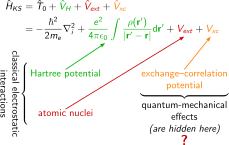
\includegraphics[width=0.7\linewidth]{figures/H.pdf}
   \end{center}
\end{frame}

\begin{frame}
   \frametitle{Exchange--correlation functionals}
   \begin{itemize}
      \item LDA -- local density approximation, $V_\mathrm{xc}^\mathrm{LDA}(n(\vec{r}))$
      \item GGA -- generalized gradient approximation, $V_\mathrm{xc}^\mathrm{LDA}(n(\vec{r}), \nabla n(\vec{r}))$
      \item Meta GGA -- also include the second derivation of the density
      \item LDA/GGA + U -- Hubbard correction for strongly correlated electrons
      \item Hybrid functionals (hf) -- mixing Hartree-Fock with LDA or GGA
      \item Many body approaches -- mainly based on GW approximation 
   \end{itemize}
   
   \pause
   \hspace{1.1cm} LDA \hspace{1.6cm} GGA (PBE) \hspace{1cm} metaGGA (mBJ) \hspace{1cm} hf (B3LYP)

   \hspace{-0.4cm}
   \includegraphics[width=0.26\linewidth]{figures/LDA.pdf}
   \hspace{0.05cm}
   \includegraphics[width=0.242\linewidth]{figures/PBE.pdf}
   \hspace{0.05cm}
   \includegraphics[width=0.242\linewidth]{figures/mBJsp.pdf}
   \hspace{0.05cm}
   \includegraphics[width=0.242\linewidth]{figures/hf.pdf}

   \hspace{0.6cm} $E_\mathrm{g}=0.47$\,eV \hspace{1cm} $E_\mathrm{g}=0.58$\,eV \hspace{1cm} $E_\mathrm{g}=1.17$\,eV \hspace{1cm} $E_\mathrm{g}=1.16$\,eV
\end{frame}

\begin{frame}
   \frametitle{Self-consistent density}
   \vspace{0.7cm}
   \begin{center}
      \includegraphics[width=0.7\linewidth]{figures/scf.pdf}
   \end{center}
\end{frame}

\subsection{Calculation of optical properties}
\begin{frame}
   \frametitle{Electronic transitions}
   \vspace{-0.2cm}
   \begin{block}{Bethe-Salpeter equation (BSE)}
      In the BSE formalism, one solves the eigenvalue problem for the effective Hamiltonian
      $$ H ^{\rm (eff)}\: | A_{\lambda} \rangle= E_{\lambda}\: |A_{\lambda}\rangle $$
   $$ H ^{\rm (eff)} = H ^{\rm (diag)}+2\:H ^{\rm (x)} + H ^{\rm (c)} $$
   \end{block}
   \begin{itemize}
      \item The diagonal term of the Hamiltonian, $H^{\rm (diag)}$, accounts for the contribution of single-particle transitions
   $$ H^{\rm (diag)}_{v\,c\,\vec{k},\,v'c'\vec{k'}} = (\epsilon_{c\,\vec{k}} - \epsilon_{v\,\vec{k}}) \:\delta_{v\,v'}\:\delta_{c\,c'}\:\delta_{\vec{k\,k'}} $$
      \item The exchange term $H^{\rm (x)}$ is caused by the repulsive interaction between the electron and the hole
   $$ H^{\rm (x)}_{v\,c\,\vec{k},\,v'c'\vec{k'}} = \int \!\!d^{3}\vec{r}\!\!\int\!\! d^{3}\vec{r'} \:\phi_{v\,\vec{k}}(\vec{r})\: \phi_{c\,\vec{k}}^* (\vec{r})\: \overline{v}(\vec{r,r'}) \:\phi^*_{v'\vec{k'}}(\vec{r'})\: \phi_{c'\vec{k'}} (\vec{r'}) $$
      \item The correlation term contains the attractive electron-hole correlation, due to the screened Coulomb potential $W(\vec{r},\vec{r'})$
$$ H^{\rm (c)}_{v\,c\,\vec{k},\,v'c'\vec{k'}} = -\int\!\! d^{3}\vec{r}\!\!\int\!\! d^{3}\vec{r'}\: \phi_{v\,\vec{k}}(\vec{r})\: \phi_{c\,\vec{k}}^* (\vec{r'}) \:W(\vec{r,r'}) \:\phi_{v'\vec{k'}}^*(\vec{r}) \:\phi_{c'\vec{k'}} (\vec{r'}) $$
   $$ \operatorname{Im} \left[\varepsilon_{\!M}(\omega)\right] = \dfrac{8\pi^2}{V}\sum_{\lambda}\: |t_{\lambda}|^2\:\delta(\omega - E_{\lambda}) \hspace{1cm}
   t_{\lambda}=\sum_{v\,c\,\vec{k}}\:A^{\lambda}_{v\,c\,\vec{k}}\: \dfrac{\langle v\,\vec{k}|\hat{\vec{p}}|c\,\vec{k}\rangle}{\epsilon_{c\,\vec{k}} - \epsilon_{v\,\vec{k}}} $$
   \end{itemize}
\end{frame}

\begin{frame}
   \frametitle{Electronic transitions}
   \framesubtitle{Applied to broad range of materials}
   \vspace{-0.7cm}
   \begin{columns}
      \begin{column}{0.5\textwidth}
         \begin{center}
            \only<1->{
            Ionic compounds (MgF$_2$)\\
            \includegraphics[width=0.75\linewidth]{figures/MgF2.png}\\
            {\scriptsize Yi et al. J. Phys. Condens. Matter 24, 85602 (2012)}\\
            \vspace{0.2cm}
            }
            \only<3->{
            Semiconductors (GaAs)\\
            \includegraphics[width=0.60\linewidth]{figures/GaAs.pdf}\\
            {\scriptsize Rohlfing et al. Phys. Rev. Lett. 81, 2312 (1998)}
            }
         \end{center}
      \end{column}
      \begin{column}{0.5\textwidth}
         \begin{center}
            \only<2->{
            Metals (Au)\\
            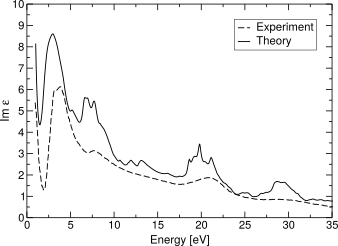
\includegraphics[width=0.75\linewidth]{figures/Au.pdf}\\
            {\scriptsize Ambrosch-Draxl et al. Comput. Phys. Commun. 175, 1--14 (2006)}\\
            \vspace{0.2cm}
            }
            \only<4->{
            Oxides (TiO$_2$)\\
            \includegraphics[width=0.65\linewidth]{figures/TiO2.png}\\
            {\scriptsize Landmann et al. J. Phys. Condens. Matter 24, 195503 (2012)}\\
            \vspace{0.5cm}
            }
         \end{center}
      \end{column}
   \end{columns}
\end{frame}

\begin{frame}
   \frametitle{Lattice vibrations}
   \begin{block}{Phonons}
      \begin{itemize}
         \item Finite displacement elements method -- atoms are displaced by a small amount from their equilibrium positions and resulting forces are used to build the dynamical matrix
         \item Density functional perturbation theory -- atomic displacement as a perturbation, many physical properties are derivatives of the total energy(or a suitable thermodynamic potential) with respect to perturbations.
      \end{itemize}
   \end{block}
   \begin{center}
      \includegraphics[width=0.65\linewidth]{figures/phonons.png}\\
      {\scriptsize Wei et al. Phys. Rev. B 50, 2221--2226 (1994)}\\   
   \end{center}
\end{frame}
%FIXME: physical properties as a 

\section{\TiSiO{} showcase}

\begin{frame}
   \frametitle{\TiSiO{} showcase}
   \begin{columns}
      \begin{column}{0.6\textwidth}
         \vspace{1cm}
         \begin{itemize}
            \item Big difference between optical and electronic properties
            \item Refractive index: TiO$_2$ $>$2.5, SiO$_2$ $\sim$1.5
            \item Band gap: TiO$_2$ 3.0--3.5\,eV, SiO$_2$ $\sim$9\,eV
            \item Static dielectric function TiO$_2$ $\sim$80, SiO$_2$ $\sim$3.9
            \item Fine-tuning properties by composition change brings new possibilities in design of optical devices (filters, anti-reflective coatings, ...)
            \item Experimentally quite well known system -- benchmark for methodology testing
         \end{itemize}
      \end{column}
      \begin{column}{0.4\textwidth}
         \begin{center}
            TiO$_2$
            \includegraphics[width=\linewidth]{figures/SEM-Xsection-TiO2.png}
            \vspace{0.3cm}
            SiO$_2$
            \includegraphics[width=\linewidth]{figures/SEM-Xsection-SiO2.png}
         \end{center}
      \end{column}
   \end{columns}
\end{frame}

\subsection{Modelling}
\begin{frame}
   \frametitle{Construction of structural models}
   \vspace{-0.3cm}
   \begin{columns}
      \begin{column}{0.8\textwidth}
         \begin{itemize}
            \item Density Functional Theory
            \item Vienna Ab initio Simulation Package (pseudopotential plane wave DFT code)
            \item Standard GGA PBE exchange-correlation functional
            \item Structure sizes around 100 atoms
         \end{itemize}
      \end{column}
      \begin{column}{0.2\textwidth}
         \begin{center}
            \includegraphics[width=0.9\linewidth]{figures/VASP.jpg}
         \end{center}
      \end{column}
   \end{columns}

   \pause

   \begin{columns}
      \begin{column}{0.5\textwidth}
         \begin{center}
             \includegraphics[width=0.6\linewidth]{figures/SQS.png}
         \end{center}
         \begin{itemize}
            \item Crystalline solid solutions with Special Quasirandom Structures (SQS) methods
            \item Based on anatase, rutile and selected SiO$_2$ structures
         \end{itemize}
      \end{column}

      \pause

      \begin{column}{0.5\textwidth}
         \begin{center}
            \includegraphics[width=0.5\linewidth]{figures/am-SA.png}
         \end{center}
         \begin{itemize}
            \item Amorphous structures prepared by ab-initio simulated annealing (SA)
            \item Annealed at 3000\,K for 3\,ps than cooled to 0K over 3\,ps and relaxed
         \end{itemize}
      \end{column}
   \end{columns}
\end{frame}

\begin{frame}
   \frametitle{Structural stability}
   \begin{columns}
      \begin{column}{0.55\textwidth}
         \vspace{-0.5cm}
         \begin{center}
            \includegraphics[width=\linewidth]{figures/Ef-all.pdf}
         \end{center}
      \end{column}
      \begin{column}{0.45\textwidth}
         \begin{center}
            \only<1-2>{
               \includegraphics[width=0.7\linewidth]{figures/coord.pdf}
            }
            \only<3>{
               \includegraphics[height=4cm]{figures/phase.png}
            }
         \end{center}
      \end{column}
   \end{columns}

   \begin{itemize}
      \item SiO$_2$ like structures are more preferable (4-coordinated tetrahedral position)
      \item Amorphous structures less stable (at 0K)
      \item<2-> Known problem with TiO$_2$ stable structure prediction for both LDA and GGA 
      \item<2-> LDA+U/GGA+U helps\footnotemark, as well as hybrid or GW
      \item<3> Preference for separate phases, in agreement with phase diagram\footnotemark
   \end{itemize}
   \footnotetext[1]{Vu, N. H. et al., J. Phys. Condens. Matter 24, 405501 (2012).}
   \only<3>{
      \footnotetext[2]{\url{http://materials.springer.com/isp/phase-diagram/docs/c_0201188}}
   }
\end{frame}

\subsection{Band gap problems}
\begin{frame}
   \frametitle{Band gap problem}
   \framesubtitle{How to get a band gap cosistent with experiment}

   \vspace{-0.2cm}
   Notorious DFT (LDA/GGA) problem in band gap underestimation
   \begin{itemize}
      \item Possible ways to fix include scissor operator, DFT+U, hybrid and many body perturbation theory based approaches
      \item Hybrids and GW not feasible for large cells
   \end{itemize}

   \pause

   \emph{TB-mBJ exchange potential}$^1$ in combination with LDA-correlation offers solution
   \begin{itemize}
      \item<2-> Contains empirical parameters tuned for band gap value on large set of solids 
      \item<3-> Was already tested for optical properties of pure TiO$_2$ and found in reasonable agreement$^2$
      \item<3-> Improved TB-mBJ parametrisations$^3$ offer even better experimental agreement
      \item<3-> TB-mBJ and optical calculations done in Wien2k (all electron full-potential DFT code)
   \end{itemize}

   \only<2>{
      \vspace{-1.8cm}
      \begin{center}
         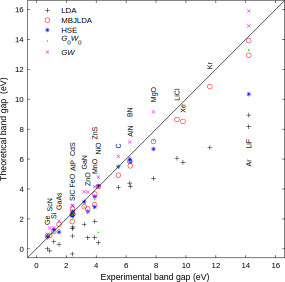
\includegraphics[width=4.65cm]{figures/mBJ.pdf}
      \end{center}
   }
   
   \only<2->{
      \footnotetext[1]{Tran, F. \& Blaha, P., Phys. Rev. Lett. 102, 226401 (2009).}
   }
   \only<3->{
      \footnotetext[2]{Gong, S. \& Liu, B.-G., Chinese Phys. B 21, 057104 (2012).}
      \footnotetext[3]{Koller, D., Tran, F. \& Blaha, P., Phys. Rev. B 85, 155109 (2012).}
   }
\end{frame}

\begin{frame}
   \frametitle{Band gap evolution}
   \framesubtitle{What happens when we add silicon into titania}

   \begin{columns}
      \begin{column}{0.5\textwidth}
         \begin{center}
            \includegraphics[width=\linewidth]{figures/gap1.pdf}
            \only<2->{
               \includegraphics[width=0.8\linewidth]{figures/SiTiO2-dos.pdf}
            }
         \end{center}
      \end{column}
      \begin{column}{0.5\textwidth}
         \begin{itemize}
            \item Band gap (HOMO-LUMO like) actually decreases when Si is added
            \item This is observable for all structures
            \item<2-> States appear below and above the valence band
            \item<3> Si-induced oxygen states
         \end{itemize}
         \begin{center}
            \only<3>{
               \includegraphics[width=0.6\linewidth]{figures/localisation.png}
            }
         \end{center}
      \end{column}
   \end{columns}
\end{frame}

\begin{frame}
   \frametitle{Band gap evolution}
   \framesubtitle{How to filter out the localized defect states}

   \begin{columns}
      \begin{column}{0.5\textwidth}
         Localized states observed also in the amorphous structures near the edge of valence and conduction band
         \begin{center}
            \includegraphics[width=\linewidth]{figures/IPR.pdf}
         \end{center}
      \end{column}
      \pause
      \begin{column}{0.5\textwidth}
         Band gap without localized states was estimated by an approach similar to Tauc plot
         \begin{center}
            \includegraphics[width=\linewidth]{figures/gap-edge.pdf}
         \end{center}
      \end{column}
   \end{columns}
\end{frame}

\subsection{Experimental setup}

\begin{frame}
   \frametitle{Deposition and characterisation}

   \begin{columns}
      \begin{column}{0.5\textwidth}
         Deposition
         \begin{itemize}
         \item \TiSiO{} thin films deposited by PECVD on c-Si
         \item Precursor gasses Titanium isopropoxide and Hexamethyldisiloxane
         \item<2-> ICP PECVD reactor, $p = 3$\,mTorr, $P = 400$\,W
      \end{itemize}
      \only<1>{
         \begin{center}
            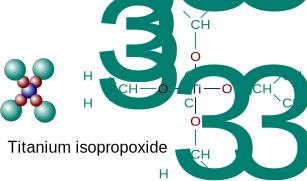
\includegraphics[width=0.6\linewidth]{figures/TTIP.pdf}
            \vspace{0.4cm}
            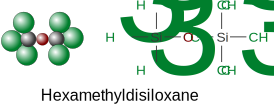
\includegraphics[width=0.6\linewidth]{figures/HMDSO.pdf}
         \end{center}
      }
      \only<2->{
         \begin{center}
            \includegraphics[width=1.0\linewidth]{figures/PECVD-reactor.pdf}
         \end{center}
      }
      \end{column}
      \begin{column}{0.5\textwidth}
         \only<3>{
            Optical characterisation
            \begin{itemize}
               \item Characterization done in spectral region up to 8.7eV
               \item Variable angle ellipsometry
               \item So-called Universal dispersion model was used$^1$
               \item Roughness (Rayleigh-Rice theory) and inhomogeneity included in the structural model
               \item NewAD fitting software
            \end{itemize}
            Composition and stochiometry determined by XPS, crystallinity by XRD
         }
         \end{column}
   \end{columns}
   \only<3>{
      \footnotetext[1]{Franta, D., Nečas, D. \& Ohlídal, I., Appl. Opt. 54, 9108 (2015).}
   }
\end{frame}

\subsection{Optical properties}

\begin{frame}
   \frametitle{Dielectric function}

   \begin{columns}
      \begin{column}{0.3\textwidth}
         \begin{itemize}
            \item Dielectric function calculated with Wien2k optic module 
            \item Calculation at the Random Phase Approximation level, e.g. no excitonic effects
            \item Good match of intensity, slight shift of peaks maxima
         \end{itemize}
      \end{column}
      \begin{column}{0.7\textwidth}
         \begin{center}
            \includegraphics[width=\linewidth]{figures/epsi.pdf}
            \newline
            \includegraphics[width=\linewidth]{figures/epsi-calc.pdf}
         \end{center}
      \end{column}
   \end{columns}
\end{frame}

\begin{frame}
   \frametitle{Band gap}
   \framesubtitle{Comparison with experiment}

   \begin{center}
      \only<1>{
         \includegraphics[width=0.6\linewidth]{figures/gap2.pdf}
      }
      \only<2>{
         \includegraphics[width=0.6\linewidth]{figures/gap3.pdf}
      }
   \end{center}

   \begin{itemize}
      \item Experimental optical band gap increases slowly from value 3.26\,eV for pure TiO$_2$ and only after $x = 0.5$ goes up more sharply to $\sim$8.0\,eV for pure SiO$_2$
      \item<2> Almost perfect agreement for the calculated band gap of a-\TiSiO{} with experimental optical band gap after filtering out the localized states near band edges
   \end{itemize}
\end{frame}

\begin{frame}
\frametitle{Refractive index}
   \begin{columns}
      \begin{column}{0.7\textwidth}
         \vspace{-0.4cm}
         \begin{center}
            \includegraphics[width=0.8\linewidth]{figures/SiTiO2-n.pdf}

            \only<2>{
               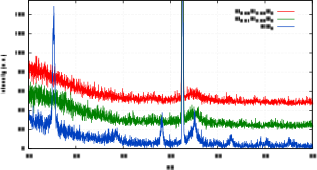
\includegraphics[width=0.7\linewidth]{figures/XRD.png}
            }
         \end{center}
      \end{column}
      \begin{column}{0.3\textwidth}
            \begin{itemize}
               \item Refractive index decreases approximately linearly in whole composition range
               \item Perfect agreement with experimental refractive index for a-\TiSiO{} again
               \item<2> By comparison with XRD we confirm the film are indeed amorphous except for pure TiO$_2$ where we have an anatase phase.
            \end{itemize}
      \end{column}
   \end{columns}
\end{frame}

\subsection{Phase separation problem}
\begin{frame}
   \frametitle{Phase separation problem}
   \vspace{-0.45cm}
   \begin{block}{X-ray photoelectron spectroscopy modelling}
      \begin{itemize}
         \item Phase separation into TiO$_2$/SiO$_2$ domains observed with samples deposited under energetic bombardment
         \item Could be quantified by fitting the O1s peak into Ti--O--Ti, Ti--O--Si and Si--O--Si parts
         \item Fitting is ambiguous without some constraints due to the broad nature of the individual peaks
         \item Core electron binding energy was calculated for every O atom in the amorphous structure, producing simulated XPS spectra
      \end{itemize}
   \end{block}
   \begin{center}
      \only<1>{\includegraphics[width=0.35\linewidth]{figures/XPSexp.pdf}
      \hspace{0.2cm}\vspace{-1cm}   
      \includegraphics[width=0.37\linewidth]{figures/XPSfit.pdf}}
      \only<2>{\includegraphics[width=0.35\linewidth]{figures/XPSexp.pdf}
      \hspace{0.2cm}\includegraphics[width=0.335\linewidth]{figures/XPScalc.pdf}}
      \only<3>{\includegraphics[width=0.33\linewidth]{figures/XPSfit.pdf}
      \hspace{0.2cm}
      \includegraphics[width=0.37\linewidth]{figures/XPSdeconv.pdf}}
   \end{center}

\end{frame}

\section{Getting started}
\begin{frame}
   \frametitle{How to get started}
   \begin{block}{Software}
      \begin{itemize}
         \item There are tens of {\it ab initio} codes around, some even licensed under GPL or some other open source license
         \item Majority of them have excellent documentation and a community willing to help newcomers.
         \item Unfortunately lots of codes only supports UNIX-like systems.
      \end{itemize}
   \end{block} 

   \pause

   \begin{block}{Hardware}
      \begin{itemize}
         \item Simple systems (few atoms) can be computed on your laptop
         \item For bigger systems (tens of atoms) or more demanding calculations (GW, full BSE) better hardware is needed
         \item Nowadays you can get reasonable machine (8 cores, 64GB memory) for less than 1200\,€
         \item Many opportunities to get CPU time at supercomputing centers if you are serious about this.
      \end{itemize}
   \end{block}
\end{frame}

\begin{frame}
   \frametitle{Software}
   \begin{center}
      \includegraphics[width=\linewidth]{figures/wiki.png}
   \end{center}
\end{frame}

\begin{frame}
   \frametitle{Software}
   \begin{center}
      \includegraphics[width=\linewidth]{figures/w2w.png}
   \end{center}
\end{frame}

\section{Conclusions}
\begin{frame}
   \frametitle{Conclusions and acknowledgment}
   \begin{block}{{\it Ab initio} modeling techniques}
      \begin{itemize}
         \item {\it Ab initio} calculations are very helpful tool when theoretical insight is needed 
         \item Can be used to explain observed features and trends in known materials
         \item Can be used to predict behavior and properties of new materials, saving time and money for experiments
         \item Just tiny example of what {\it ab initio} techniques can do today
      \end{itemize}
   \end{block}

   \only<2->{
      \begin{center}
         \emph{Acknowledgment}
      \end{center}
   
      \begin{columns}
         \begin{column}{0.3\textwidth}
            Montanuniversität Leoben
            \begin{itemize}
               \item David Holec
            \end{itemize}
         \end{column}
         \begin{column}{0.3\textwidth}
            Masaryk University
            \begin{itemize}
               \item David Nečas
               \item Daniel Franta
               \item Marek Eliáš
               \item Eva Kedroňová
               \item Lenka Zajíčková
            \end{itemize}
         \end{column}
         \begin{column}{0.3\textwidth}
            Université de Nantes
            \begin{itemize}
               \item Stéphane Elisabeth
               \item Antoine Goulet
               \item Mireille Richard
               \item Agnes Granier
            \end{itemize}
         \end{column}
      \end{columns} 
   }
   \vspace{0.5cm}
   \only<3>{
      \begin{center}
         \emph{Thank you for your attention.}
      \end{center}
   }

\end{frame}



\end{document}
